\begin{bx1}
    内径が$a$である中空の導体球の表面がいくつかの平板の組によって
    \emph{偶数}個の等しい部分に分けられている;平板の交線は$z$軸と一致しており,
    平板は角度$\phi$の等しい間隔で分布しているとする.(各部分はりんごをくし切りにしたときの
    皮のようなもの,あるいは連続する経線の間の地球の表面のようなものである.)これらの
    各部分のポテンシャルは交互に$\pm V$であるとして一定であるとする.
    \begin{enumerate}[(a)]%  
      \item 球体内部のポテンシャルに対する級数展開を
        一般の$2n$個に分けた区間について計算せよ.ただし,どの係数が非ゼロであるかを
        正確に決定し,非ゼロの結果が得られる場合については,その結果を$\cos\theta$
        についての積分で表示せよ.
      \item $n = 1$の特別な場合(2つの半球)について,$l = 3$までの項を明示せよ.
        また,座標軸を適当にとることで,3.3節の(3.36)の結果が得られることを確認せよ.
    \end{enumerate}%
  \end{bx1}
  \begin{wrapfigure}[14]{r}{0.2\linewidth} 
    \centering
    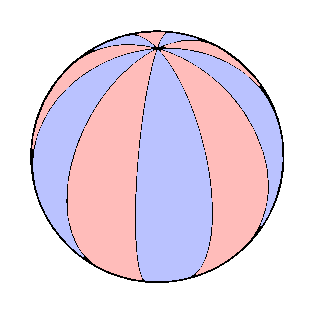
\includegraphics[width=\linewidth]{fig/Jackson3-4_1.pdf}\\
    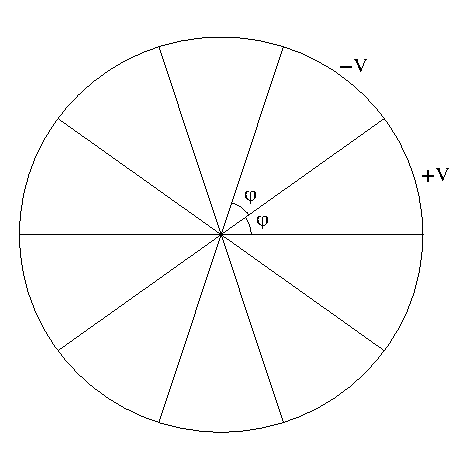
\includegraphics[width=\linewidth]{fig/Jackson3-4_2.pdf}
  \end{wrapfigure}%
\itemlabel{(a)}
  球内部でのポテンシャルは,原点での特異性に気をつけると,
  \begin{gather}%  
    \label{eq:3-4_eq1}
    \Phi(r,\theta,\phi) = \sum_{l=0}^\infty \sum_{m=-l}^{l} A_{lm}r^l Y_{lm}(\theta,\phi)
  \end{gather}%
  と書くことができる.
  境界条件は,
  \begin{multline}%
    \Phi(r=a,\theta,\phi) \equiv V(\phi)=
    \begin{dcases}%
      +V \qqtext{if} \frac{\pi}{n} \cdot 2j \leq \phi \leq \frac{\pi}{n}\cdot(2j+1)\\
      -V \qqtext{if} \frac{\pi}{n}\cdot(2j+1) \leq \phi \leq \frac{\pi}{n}\cdot (2j+2)
    \end{dcases}\\%
    \qqtext{for} j = 0, 1, \ldots, n-1
  \end{multline}%
  である.
  \begin{gather}%
    V(\phi) = \sum_{l} \sum_{m} A_{lm} a^l Y_{lm}(\theta,\phi)
  \end{gather}%
  に対して,両辺に$Y^*_{l'm'}(\theta,\phi)$をかけて,
  $\dl{\Omega} = \sin\theta\dl{\theta,\phi}$で積分を実行すると,
  球面調和関数の直交性より
  \begin{align}%
    A_{lm} &= \frac{1}{a^l} \int V(\phi) Y^*_{lm}(\theta,\phi) \dl{\Omega}\notag\\
    &= \frac{1}{a^l} \sqrt{\frac{2l+1}{4\pi}\frac{(l-m)!}{(l+m)!}}\int_0^\pi
    P_{l}^m(\cos\theta)\sin\theta\dl{\theta} \int_0^{2\pi} V(\phi) \e^{-\i m\phi}\dl{\phi}
  \end{align}%
  である.$\phi$での積分について,
  \begin{gather}
    \int_0^{2\pi} V(\phi) \e^{-\i m\phi} \dl{\phi} = V \sum_{j=0}^{n-1} \ab[
      \int_{\frac{\pi}{n}2j}^{\frac{\pi}{n}(2j+1)} \e^{-\i m\phi}\dl{\phi}
      - \int_{\frac{\pi}{n}(2j+1)}^{\frac{\pi}{n}(2j+2)} \e^{-\i m\phi}\dl{\phi}
    ]
  \end{gather}
  となるが, $m = 0$のとき,
  \begin{gather}%
    \int_0^{2\pi} V(\phi)\e^{-\i m\phi} \dl{\phi} =  0
  \end{gather}%
  であり,$m \neq 0$のときは
  \begin{gather}%
    \int_0^{2\pi} V(\phi) \e^{-\i m\phi} \dl{\phi} =
    - \frac{\i V}{m} \ab(1-\e^{-\i \frac{m}{n}\pi})^2 \sum_{j=0}^{n-1}\ab(\e^{-\i \frac{2m}{n}\pi})^j
  \end{gather}%
  となるが,$\exp(-\i (m/n)\pi) = 1$つまり$m/(2n)$が整数となるときはゼロとなる.
  また,
  \begin{gather}%
    \sum_{j=0}^{n-1} \ab(\e^{-\i\frac{2m}{n}\pi})^j 
    = \frac{1 - \e^{-\i 2m\pi}}{1-\e^{\i \frac{2m}{n}\pi}}
  \end{gather}%
  となるので,$m/n$が整数となるときには右辺が$0 / 0$の形になるので,non-zeroとなることが
  期待される.一方,それ以外の場合では$m$が整数であることより分子がゼロになるので,
  この和はゼロである.
  以上をまとめると,$m / n = \pm1, \pm3, \ldots$の場合のみが
  non-zeroの結果を与えることがわかる.実際,このときは
  \begin{gather}%  
    \int_0^{2\pi} V(\phi) \e^{-\i m\phi} \dl{\phi} =
    -\frac{\i V}{m}\ab(1-(-1))^2 \sum_{j=0}^{n-1} 1 = -4\i V \frac{n}{m}
  \end{gather}%
  である.
  以上の結果を踏まえると,球内部でのポテンシャルを\eqref{eq:3-4_eq1}のように展開したとき,
  係数$A_{lm}$は
  \begin{gather}%
    A_{lm} = 
    \begin{dcases}%
      \begin{multlined}
        -\frac{4\i V}{a^l}\frac{n}{m} \sqrt{\frac{2l+1}{4\pi}\frac{(l-m)!}{(l+m)!}} 
        \int_{-1}^1 P_l^m (\cos\theta)\dl{(\cos\theta)} \\
        \qqtext{if} m = \pm n, \pm 3n, \pm 5n, \ldots
      \end{multlined}\\
      0 \qqtext{otherwise}
    \end{dcases}%
  \end{gather}%

\itemlabel{(b)}
  $n = 1$として係数$A_{lm}$を$l = 3$まで計算する.$m = \pm 1, \pm 3, \ldots$に対して
  $A_{lm} \neq 0$であることに注意する.
  \begin{gather*}%
    A_{1,\pm 1} = \frac{\i V}{a}\sqrt{\frac{3\pi}{2}},\qq
    A_{2,\pm 1} = 0\\
    A_{3,\pm 3} = \frac{\i V}{a^3} \sqrt{\frac{35\pi}{256}},\qq
    A_{3,\pm 1} = \frac{\i V}{a^3} \sqrt{\frac{21\pi}{256}}
  \end{gather*}%
  と計算できるので,ポテンシャルは
  \begin{gather}%
    \Phi(r,\theta,\phi) = V\left[
      \frac{3r}{2a} \sin\theta\sin\phi
      +
      \ab(\frac{r}{a})^3\ab\{
        \frac{35}{64}\sin^3\theta\sin(3\phi) + 
        \frac{21}{64}\sin\theta\ab(5\cos^2\theta-1)\sin\phi
      \} + \cdots
      \right]
  \end{gather}%
  とかける.ここで,$\cos\theta' = \sin\theta \sin\phi$とおけば,
  \begin{gather}%
    P_1(\cos\theta') = \sin\theta\sin\phi\\
    P_3(\cos\theta') = -\frac{1}{8}\ab[5\sin^3\theta\sin(3\phi) 
    + 3\sin\theta(5\cos^2-1)\sin\phi]
  \end{gather}%
  であるから,
  \begin{gather}%
    \Phi(r,\theta') = V\ab[\frac{3}{2} \frac ra P_1(\cos\theta') - 
    \frac{7}{8}\ab(\frac ra)^3P_3(\cos\theta') + \cdots]
  \end{gather}%
  となり,これは,教科書本文中の式(3.36)と一致していることがわかる.
  図\ref{fig:3-4_n3}には$n = 3$の場合の図を描いた.
  \begin{figure}[htbp]%  
    \centering%  
    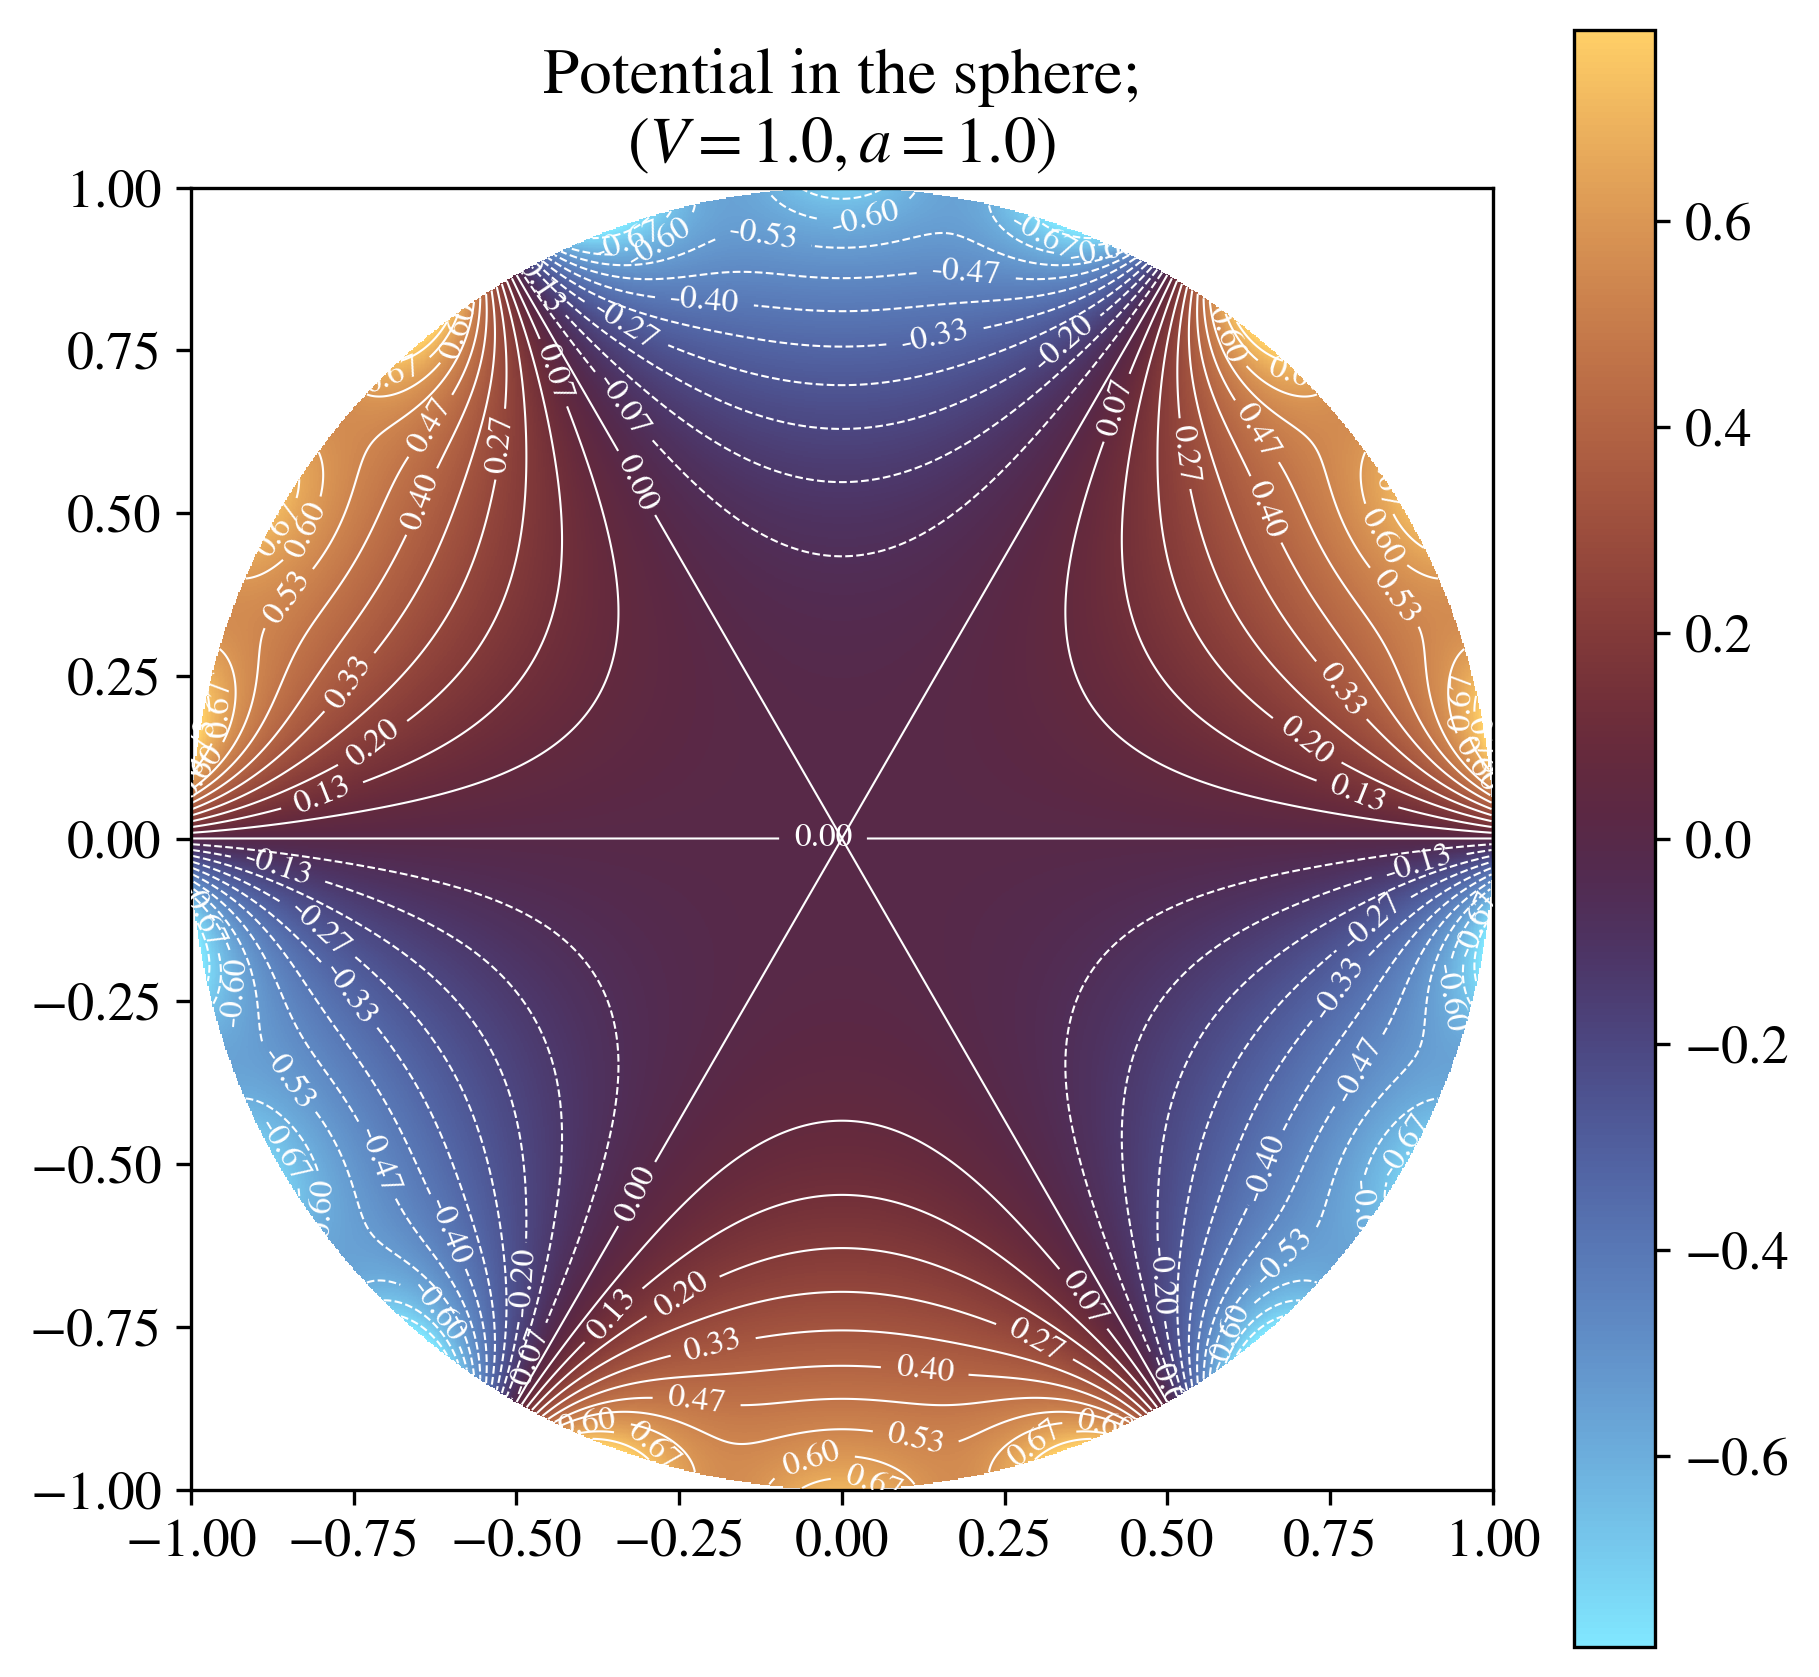
\includegraphics[width=0.5\linewidth]{py/3-4_n3.png}%  
    \caption{問題文と同じセットアップを行って,$n = 3$の場合について,$l = 20$の
    項まででポテンシャルを描いた図.球($z = 0$面で切断したときの円)の境界
    の近くでは有限項で打ち切った事による誤差が見られるが,概ね期待されるポテンシャルの
    形を得られていることがわかる.}%  
    \label{fig:3-4_n3}%  
  \end{figure}%

  \clearpage
